\documentclass[11pt,a4paper]{article}
\usepackage[margin=21mm,headheight=16pt]{geometry}
\usepackage{fontspec}\setmainfont{Noto Serif}\setsansfont{Noto Sans}\setmonofont{Noto Sans Mono}
\usepackage{polyglossia}\setdefaultlanguage{turkish}
\usepackage{amsmath,amssymb,mathtools,graphicx,xcolor,booktabs,tabularx,array,enumitem}
\usepackage[most]{tcolorbox}\usepackage{fancyhdr,titlesec,needspace}
\usepackage[unicode,hidelinks,breaklinks]{hyperref}\usepackage{bookmark}
\definecolor{ink}{HTML}{18233A}\definecolor{accent}{HTML}{545AC4}\definecolor{green}{HTML}{087E66}\definecolor{paper}{HTML}{F3F5FA}
\color{ink}\setlength{\parindent}{0pt}\setlength{\parskip}{7pt}\linespread{1.10}
\setlength{\emergencystretch}{3em}\allowdisplaybreaks
\setlist{topsep=4pt,itemsep=4pt,leftmargin=*}
\pagestyle{fancy}\fancyhf{}\fancyhead[L]{\sffamily\small MÜHENDİSLİK MATEMATİĞİ}\fancyhead[R]{\sffamily\small Ders çalışma notları}\fancyfoot[L]{\sffamily\scriptsize Fotoğraflar + müfredat | 8 Kasım 2026}\fancyfoot[R]{\sffamily\thepage}
\titleformat{\section}{\Large\sffamily\bfseries\color{accent}}{\thesection}{.6em}{}
\titleformat{\subsection}{\large\sffamily\bfseries}{\thesubsection}{.6em}{}
\tcbset{enhanced,breakable,boxrule=.4pt,arc=2mm,left=3mm,right=3mm,top=2mm,bottom=2mm,before skip=8pt,after skip=8pt,fonttitle=\sffamily\bfseries,colback=paper,colframe=accent,coltitle=white}
\newcommand{\notebox}[2]{\begin{tcolorbox}[title={#1},colframe=accent!70!black]#2\end{tcolorbox}}
\hypersetup{pdfauthor={Mühendislik Matematiği Çalışma Atölyesi},pdfsubject={Ders fotoğrafları ve altı başlıklı müfredata göre özgün Türkçe çalışma notları}}
\begin{document}

\hypersetup{pdftitle={Zincir kuralı, yönlü türev ve gradyan}}
{\sffamily\small\color{accent} ÇALIŞMA ATÖLYESİ / KONU 06\par}
\vspace{8mm}
{\Huge\sffamily\bfseries\raggedright\hyphenpenalty=10000 Zincir kuralı, yönlü türev ve gradyan\par}
\vspace{3mm}
{\large Bağımlılık ağaçları, kapalı türev, değişken dönüşümleri, en hızlı artış ve seviye yüzeyine normal.\par}
\vspace{4mm}\hrule\vspace{4mm}\subsection*{Bu bölümün hedefleri}\begin{itemize}
\item Birden fazla yoldan gelen türev katkılarını zincir kuralında toplamak.
\item Kapalı denklemlerde türevleri geçerlilik koşullarıyla hesaplamak.
\item Gradyan ve birim yön kullanarak yönlü türev ve en hızlı artışı bulmak.\end{itemize}
{\small\tableofcontents}\clearpage
\section{Bağımlılık ağacı ve tek parametreli zincir kuralı}
\(z=f(x,y)\) ve \(x=x(t),y=y(t)\) ise t değişince z iki yoldan etkilenir. Her yol üzerindeki türevler çarpılır ve yollar toplanır. Önce hangi değişkenin hangisine bağlı olduğunu çizmek, eksik terimleri önler. f nin türevleri \((x(t),y(t))\) noktasında değerlendirilir.


{\small\[
\frac{dz}{dt}=f_x\frac{dx}{dt}+f_y\frac{dy}{dt},\qquad\frac{dw}{dt}=f_xx\prime(t)+f_yy\prime(t)+f_zz\prime(t).
\]}
İkinci formülde \(f_xx\prime\) ifadesi \(f_x\,x\prime\) çarpımıdır; ikinci kısmi türev \(f_{xx}\) ile karıştırılmamalıdır. Bütün ara değişkenler aynı parametreye bağlıysa d/dt kullanılır.

\Needspace{10\baselineskip}\begin{tcolorbox}[title={Örnek 6.1 | Tahtadaki trigonometrik zincir örneği},colframe=accent]\(z=x^2+y^2\), \(x=\cos t+\sin t\), \(y=\cos t-\sin t\). dz/dt nedir?
\par\vspace{1mm}{\scriptsize\sffamily Ders fotoğrafından | \nolinkurl{IMG-20261105-WA0041.jpg}}\end{tcolorbox}
\begin{tcolorbox}[title={Adım adım çözüm},colback=green!3!white,colframe=green]\begin{enumerate}
\item \(z_x=2x,z_y=2y\); \(x\prime=-\sin t+\cos t\), \(y\prime=-\sin t-\cos t\). Zincir toplamı 0 olur.
\item Doğrudan kontrol: \((\cos t+\sin t)^2+(\cos t-\sin t)^2=2\). Sabit fonksiyonun türevi 0.
\end{enumerate}\end{tcolorbox}
\Needspace{10\baselineskip}\begin{tcolorbox}[title={Örnek 6.2 | Çarpanlı fonksiyonda zincir kuralı},colframe=accent]\(z=xy\), \(x=\cos t,y=\sin t\). dz/dt yi bulunuz.
\par\vspace{1mm}{\scriptsize\sffamily Ders fotoğrafından | \nolinkurl{IMG-20261105-WA0041.jpg}}\end{tcolorbox}
\begin{tcolorbox}[title={Adım adım çözüm},colback=green!3!white,colframe=green]\begin{enumerate}
\item \(z_x=y,z_y=x\). Böylece \(z\prime=\sin t(-\sin t)+\cos t\cos t=\cos^2t-\sin^2t\).
\item Doğrudan \(z=\tfrac12\sin2t\) türevi de \(\cos2t\), aynı sonuçtur.
\end{enumerate}\end{tcolorbox}
\section{İki yeni değişkene bağlı zincir kuralı}
\(z=f(x(u,v),y(u,v))\) olduğunda u ve v bağımsız yeni değişkenlerdir. u ya göre türev alırken v sabit tutulur. Aynı dış fonksiyonun farklı iç yolları katkı verir. Daha çok ara değişken varsa her biri için bir terim eklenir.


{\small\[
\frac{\partial z}{\partial u}=f_xx_u+f_yy_u,\qquad\frac{\partial z}{\partial v}=f_xx_v+f_yy_v.
\]}
Bu formüllerde \(f_xx_u\), \(f_x\,x_u\) çarpımıdır. Matris biçimi \(D(f\circ g)=Df(g)Dg\) ile aynı düzeni ifade eder. Çarpım sırası, önce iç değişkenlerin değişimi sonra dış fonksiyonun etkisi uygulanacak biçimdedir.

\Needspace{10\baselineskip}\begin{tcolorbox}[title={Örnek 6.3 | Tahtadaki logaritma örneği},colframe=accent]\(z=\ln(x^2+y^2)\), \(x=e^u\cos v,y=e^u\sin v\). \(z_u,z_v\) nedir?
\par\vspace{1mm}{\scriptsize\sffamily Ders fotoğrafından | \nolinkurl{IMG-20261108-WA0074.jpg}}\end{tcolorbox}
\begin{tcolorbox}[title={Adım adım çözüm},colback=green!3!white,colframe=green]\begin{enumerate}
\item \(f_x=2x/(x^2+y^2)\), \(f_y=2y/(x^2+y^2)\). \(x_u=x,y_u=y,x_v=-y,y_v=x\).
\item \(z_u=2(x^2+y^2)/(x^2+y^2)=2\); \(z_v=(-2xy+2xy)/(x^2+y^2)=0\).
\item Kontrol: \(x^2+y^2=e^{2u}\), dolayısıyla \(z=2u\).
\end{enumerate}\end{tcolorbox}
\Needspace{10\baselineskip}\begin{tcolorbox}[title={Örnek 6.4 | Üç ara değişkenli ders örneği},colframe=accent]\(S=\ln(x^2+y^2+z^2)\), \(x=u+v,y=u-v,z=2\sqrt{uv}\). Pozitif u ve v için \(S_u,S_v\) bulunuz.
\par\vspace{1mm}{\scriptsize\sffamily Ders fotoğrafından | \nolinkurl{IMG-20261108-WA0077.jpg}}\end{tcolorbox}
\begin{tcolorbox}[title={Adım adım çözüm},colback=green!3!white,colframe=green]\begin{enumerate}
\item \(x_u=x_v=1,y_u=1,y_v=-1,z_u=v/\sqrt{uv},z_v=u/\sqrt{uv}\).
\item Payda \(x^2+y^2+z^2=2(u+v)^2\). Zincir toplamları \(S_u=S_v=2/(u+v)\).
\item Doğrudan \(S=\ln2+2\ln(u+v)\) aynı sonucu verir. \(u,v>0\) seçimi kökün içte türevlenmesini ve logaritmanın tanımını güvenceye alır.
\end{enumerate}\end{tcolorbox}
\section{Hem doğrudan hem dolaylı bağımlılık}
Bazen bir değişken hem f içinde doğrudan görünür hem de ara değişkenlerin içinde yer alır. Örneğin \(z=f(x,y)\), \(y=y(x)\) ise f nin x e doğrudan katkısı da eklenmelidir. Yalnızca dolaylı yolu almak bir terimi kaybettirir.


{\small\[
\frac{dz}{dx}=f_x+f_y\frac{dy}{dx}.
\]}
\Needspace{10\baselineskip}\begin{tcolorbox}[title={Örnek 6.5 | İki bağımsız yeni değişkenle karmaşık örnek},colframe=accent]\(z=e^{x/y}\), \(x=\sin u,y=u^2v\), \(u,v\ne0\). \(z_u,z_v\) yi bulunuz.
\par\vspace{1mm}{\scriptsize\sffamily Ders fotoğrafından | \nolinkurl{IMG-20261108-WA0079.jpg}}\end{tcolorbox}
\begin{tcolorbox}[title={Adım adım çözüm},colback=green!3!white,colframe=green]\begin{enumerate}
\item \(f_x=e^{x/y}/y\), \(f_y=-xe^{x/y}/y^2\). \(x_u=\cos u,x_v=0,y_u=2uv,y_v=u^2\).
\item \(z_u=e^{\sin u/(u^2v)}[\cos u/(u^2v)-2\sin u/(u^3v)]\).
\item \(z_v=-e^{\sin u/(u^2v)}\sin u/(u^2v^2)\). İç ifadeyi önce sadeleştirip türev almak da kontrol yöntemidir.
\end{enumerate}\end{tcolorbox}
\section{Kapalı fonksiyonlarda türev}
\(F(x,y)=0\) denklemi y yi açıkça çözmeden yerel olarak y(x) tanımlayabilir. F bir komşulukta sürekli birinci türevlere sahipse ve \(F_y\ne0\) ise kapalı fonksiyon teoremi bu yerel çözümü güvenceye alır. Türev alınırken y nin de x e bağlı olduğu unutulmamalıdır.


{\small\[
F_x+F_yy\prime=0\quad\Longrightarrow\quad y\prime=-\frac{F_x}{F_y},\qquad F_y\ne0.
\]}
Üç değişkende \(F(x,y,z)=0\), z yi yerel olarak z(x,y) tanımlıyorsa x türevinde y sabit, y türevinde x sabit tutulur. Sürekli birinci türevler ve \(F_z\ne0\) koşuluyla aşağıdaki formüller geçerlidir.


{\small\[
z_x=-\frac{F_x}{F_z},\qquad z_y=-\frac{F_y}{F_z}.
\]}
\Needspace{10\baselineskip}\begin{tcolorbox}[title={Örnek 6.6 | Tahtadaki kapalı türev sorusu},colframe=accent]\(2x^4z^3+3xy^2+4xz+3y+5x-23=0\) denkleminin tanımladığı z(x,y) için \((1,2)\) noktasında \(z_x,z_y\) nedir?
\par\vspace{1mm}{\scriptsize\sffamily Ders fotoğrafından | \nolinkurl{IMG-20261108-WA0081.jpg}}\end{tcolorbox}
\begin{tcolorbox}[title={Adım adım çözüm},colback=green!3!white,colframe=green]\begin{enumerate}
\item Önce z bulunur: \(2z^3+4z=0\). Gerçek çözüm \(z=0\); inceleme noktası \((1,2,0)\).
\item \(F_x=8x^3z^3+3y^2+4z+5\), \(F_y=6xy+3\), \(F_z=6x^4z^2+4x\).
\item Noktada \(F_x=17,F_y=15,F_z=4\ne0\). Böylece \(z_x=-17/4,z_y=-15/4\). Yerel z(x,y) yorumu geçerlidir.
\end{enumerate}\end{tcolorbox}
\Needspace{10\baselineskip}\begin{tcolorbox}[title={Örnek 6.7 | Kapalı denklemin teğet düzlemi},colframe=accent]\(x^2+y^2+z^2=9\) küresinin \((1,2,2)\) noktasındaki teğet düzlemi nedir?
\par\vspace{1mm}{\scriptsize\sffamily Pekiştirme}\end{tcolorbox}
\begin{tcolorbox}[title={Adım adım çözüm},colback=green!3!white,colframe=green]\begin{enumerate}
\item \(F=x^2+y^2+z^2-9\), gradyanı \((2x,2y,2z)\). Noktada normal \((2,4,4)\).
\item \(2(x-1)+4(y-2)+4(z-2)=0\), yani \(x+2y+2z=9\). Bu normal merkezden noktaya giden yarıçapla paraleldir.
\end{enumerate}\end{tcolorbox}
\section{İkinci türevde zincir kuralı}
Bir değişken dönüşümünde ikinci türev alınırken ilk zincir toplamının hem katsayıları hem türevleri değişir. Bu nedenle iç fonksiyonların ikinci türevleri de ortaya çıkar. \(x=x(t),y=y(t)\) için sürekli ikinci türevler varsayımıyla:


{\small\[
\frac{d^2z}{dt^2}=f_{xx}(x\prime)^2+2f_{xy}x\prime y\prime+f_{yy}(y\prime)^2+f_xx\prime\prime+f_yy\prime\prime.
\]}
\Needspace{10\baselineskip}\begin{tcolorbox}[title={Örnek 6.8 | Dersteki diferansiyel denklem dönüşümü},colframe=accent]\(x=e^t\) dönüşümü altında \(x^2y_{xx}+xy_x-y=0\) denklemini t değişkenine dönüştürünüz.
\par\vspace{1mm}{\scriptsize\sffamily Ders fotoğrafından | \nolinkurl{IMG-20261105-WA0042.jpg}}\end{tcolorbox}
\begin{tcolorbox}[title={Adım adım çözüm},colback=green!3!white,colframe=green]\begin{enumerate}
\item \(dt/dx=1/x\). Dolayısıyla \(y_x=y_t/x\).
\item Yeniden x türevi: \(y_{xx}=(y_{tt}-y_t)/x^2\). Burada hem \(y_t\) hem \(1/x\) türevlenir.
\item Denklem \((y_{tt}-y_t)+y_t-y=0\), yani \(y_{tt}-y=0\) olur. Dönüşüm \(x>0\) için geçerlidir.
\end{enumerate}\end{tcolorbox}
\section{Gradyan: türevleri bir vektörde toplamak}
\notebox{Müfredatı tamamlayan anlatım}{Fotoğraflarda zincir kuralı ve kapalı türev örnekleri açıkça görülüyor. Yönlü türev ve gradyan ise verilen müfredatın 6. başlığında yer alıyor; bu alt bölümler standart vektör analizi kurallarıyla tamamlandı. Aşağıdaki örnekler ders tahtasından aktarılmış sorular olarak sunulmuyor.}
Bir skaler alanın gradyanı kısmi türevlerden oluşan vektördür. Sıcaklık alanında her noktada hangi yöne gidildiğinde sıcaklığın daha hızlı arttığını anlatır. Skaler alan sayısal değer verir; onun gradyanı bir vektör alanıdır. Bu fark, birim ve boyut kontrolü için önemlidir.


{\small\[
\nabla f=(f_x,f_y),\qquad\nabla F=(F_x,F_y,F_z).
\]}
Türevlenebilirlik altında küçük bir \(\mathbf h\) yer değiştirmesi için \(f(P+\mathbf h)-f(P)\approx\nabla f(P)\cdot\mathbf h\). Böylece önceki bölümdeki tam diferansiyel, gradyanın yer değiştirmeyle skaler çarpımıdır. Gradyanın bileşenleri, koordinat eksenlerindeki değişim hızlarıdır.

\section{Yönlü türev ve yönü birimleştirme}
Kısmi türev yalnız eksenler boyunca değişimi ölçerken yönlü türev seçilen herhangi bir birim yönde birim uzunluk başına değişimi ölçer. \(\mathbf u\) birim olmak zorundadır. Yön \(\mathbf v\) olarak verilirse önce \(\mathbf v/\|\mathbf v\|\) alınır. P den Q ya yön sorulursa vektör Q-P dir.


{\small\[
D_{\mathbf u}f(P)=\lim_{h\to0}\frac{f(P+h\mathbf u)-f(P)}h=\nabla f(P)\cdot\mathbf u,\qquad\|\mathbf u\|=1.
\]}
Son eşitlik f nin P de türevlenebilirliği altında geçerlidir. Yalnızca kısmi türevlerin varlığını bilmek yeterli değildir. Birim olmayan vektörle skaler çarpım, o parametrizasyonun hızını da içerir; standart yönlü türevle aynı sayı olmayabilir.

\Needspace{10\baselineskip}\begin{tcolorbox}[title={Örnek 6.9 | Birim olmayan yönden yönlü türev},colframe=accent]\(f(x,y)=x^2y+3y\), \(P=(1,2)\), yön \(\mathbf v=(3,4)\). Yönlü türev nedir?
\par\vspace{1mm}{\scriptsize\sffamily Pekiştirme}\end{tcolorbox}
\begin{tcolorbox}[title={Adım adım çözüm},colback=green!3!white,colframe=green]\begin{enumerate}
\item \(f_x=2xy,f_y=x^2+3\). \(\nabla f(1,2)=(4,4)\).
\item Yönün normu 5; \(\mathbf u=(3/5,4/5)\). \(D_{\mathbf u}f=4(3/5)+4(4/5)=28/5\).
\item Birimleştirmeden alınan 28 sonucu, parametre hızını 5 katına çıkarır ve bu sorunun istediği birim uzunluk başına türev değildir.
\end{enumerate}\end{tcolorbox}
\Needspace{10\baselineskip}\begin{tcolorbox}[title={Örnek 6.10 | P den Q ya doğru değişim},colframe=accent]\(F(x,y,z)=x^2+y^2+z^2\), \(P=(1,0,2)\), \(Q=(3,1,4)\). P de Q yönündeki türev nedir?
\par\vspace{1mm}{\scriptsize\sffamily Pekiştirme}\end{tcolorbox}
\begin{tcolorbox}[title={Adım adım çözüm},colback=green!3!white,colframe=green]\begin{enumerate}
\item \(Q-P=(2,1,2)\), norm 3; birim yön \((2,1,2)/3\). \(\nabla F(P)=(2,0,4)\).
\item Skaler çarpım \((4+0+8)/3=4\). Sonucun pozitif olması bu yönde ilk anda alan değerinin arttığını gösterir.
\end{enumerate}\end{tcolorbox}
\section{En hızlı artış, azalış ve değişmeyen yön}
Sıfır olmayan gradyan için \(D_{\mathbf u}f=\|\nabla f\|\cos\theta\). En büyük kosinüs 1, en küçük -1 olduğundan en hızlı artış gradyan yönündedir. Gradyana dik yönlerde birinci mertebeden değişim sıfırdır. Bu, fonksiyonun o doğrultuda her uzaklıkta sabit kalacağı anlamına gelmez.


{\small\[
\max_{\|\mathbf u\|=1}D_{\mathbf u}f=\|\nabla f\|,\quad\mathbf u_{\max}=\frac{\nabla f}{\|\nabla f\|},\quad\min D_{\mathbf u}f=-\|\nabla f\|.
\]}
\Needspace{10\baselineskip}\begin{tcolorbox}[title={Örnek 6.11 | Gradyanla yön seçmek},colframe=accent]\(f=x^2+2y^2\) için P=(1,1) noktasında en hızlı artış yönü, hızı ve sıfır değişim yönü nedir?
\par\vspace{1mm}{\scriptsize\sffamily Pekiştirme}\end{tcolorbox}
\begin{tcolorbox}[title={Adım adım çözüm},colback=green!3!white,colframe=green]\begin{enumerate}
\item \(\nabla f=(2x,4y)\); P de \((2,4)\), norm \(2\sqrt5\). En hızlı artış birim yönü \((1,2)/\sqrt5\), hızı \(2\sqrt5\).
\item En hızlı azalış ters yönde ve türev \(-2\sqrt5\). Sıfır türev yönlerinden biri \((-2,1)/\sqrt5\), çünkü \((2,4)\cdot(-2,1)=0\).
\end{enumerate}\end{tcolorbox}
\notebox{Gradyan sıfırsa}{\(\nabla f(P)=\mathbf0\) ve f türevlenebilir ise tüm birim yönlerde birinci yönlü türev sıfırdır. Bu bilgi tek başına maksimum, minimum veya sabitlik göstermez; daha yüksek mertebe inceleme gerekir.}
\begin{center}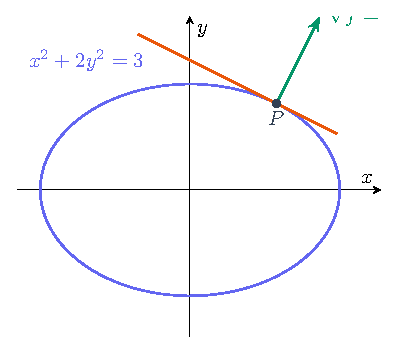
\includegraphics[width=.94\linewidth,height=65mm,keepaspectratio]{../assets/figures/gradient.pdf}\par{\small\sffamily Gradyan seviye eğrisine diktir. Birim yön gradyana döndükçe yönlü türev artar.}\end{center}
\section{Gradyan neden seviye kümesine diktir?}
\(f(x(t),y(t))=c\) seviye eğrisi boyunca sabittir. Zincir kuralıyla \(0=f_xx\prime+f_yy\prime=\nabla f\cdot\mathbf r\prime\). Dolayısıyla sıfır olmayan gradyan eğrinin teğetine diktir. Üç boyutta aynı kanıt seviye yüzeyi üzerindeki bütün teğet yönler için geçerlidir.


{\small\[
\nabla F(P)\cdot\big((x,y,z)-P\big)=0,\qquad F(P)=c,\quad\nabla F(P)\ne\mathbf0.
\]}
\Needspace{10\baselineskip}\begin{tcolorbox}[title={Örnek 6.12 | Seviye eğrisinin teğet doğrusu},colframe=accent]\(x^2+2y^2=3\) eğrisinin (1,1) noktasındaki teğeti nedir?
\par\vspace{1mm}{\scriptsize\sffamily Pekiştirme}\end{tcolorbox}
\begin{tcolorbox}[title={Adım adım çözüm},colback=green!3!white,colframe=green]\begin{enumerate}
\item Gradyan \((2,4)\) teğete normaldir. \(2(x-1)+4(y-1)=0\), yani \(x+2y=3\).
\item Bu doğrultu önceki örnekteki sıfır yönlü türev doğrultusuyla aynıdır. Teğet doğrusu eğriye yalnızca yerel olarak yaklaşır.
\end{enumerate}\end{tcolorbox}
\section{Bütün konuları bağlayan çözüm stratejisi}
\begin{enumerate}
\item Değişkenlerin bağımlılıklarını önce yaz; her bağımsız yolun katkısını ekle.
\item Kapalı türevde önce noktayı tamamla, sonra paydadaki türevin sıfır olmadığını denetle.
\item Yönlü türevde yönü birimleştir; türevlenebilirlik koşulunu kontrol et.
\item En hızlı artış yön sorusudur, en hızlı artış hızı ise norm sorusudur.
\item Seviye yüzeyinde gradyanı normal olarak kullan; noktanın yüzeyde olduğunu doğrula.
\end{enumerate}
\Needspace{10\baselineskip}\begin{tcolorbox}[title={Örnek 6.13 | Birleşik pekiştirme},colframe=accent]\(f(x,y)=e^{x-y}\), P=(0,0). P de teğet düzlem, \((1,1)\) yönünde türev ve en hızlı artış yönünü bulunuz.
\par\vspace{1mm}{\scriptsize\sffamily Pekiştirme}\end{tcolorbox}
\begin{tcolorbox}[title={Adım adım çözüm},colback=green!3!white,colframe=green]\begin{enumerate}
\item \(f(P)=1,\nabla f(P)=(1,-1)\). Grafik üzerindeki teğet düzlem \(z=1+x-y\).
\item Birim yön \((1,1)/\sqrt2\); yönlü türev 0. En hızlı artış yönü \((1,-1)/\sqrt2\), artış hızı \(\sqrt2\).
\item \(x=y\) doğrusu üzerinde fonksiyon gerçekten 1 dir. Bu örnekte sıfır türev sabit seviye doğrultusuna karşılık gelir; her fonksiyonda böyle küresel bir sonuç çıkarılmaz.
\end{enumerate}\end{tcolorbox}

\clearpage
\section*{Kaynaklar ve kapsam}
\addcontentsline{toc}{section}{Kaynaklar ve kapsam}
Bu metin 156 ders/defter fotoğrafı ve altı başlıklı müfredata göre özgün olarak yazıldı. Fotoğraflar dersin sıra ve örneklerini belirler. Ek sorular pekiştirme olarak etiketlidir; çıkmış sınav sorusu iddiası yoktur. Soluk semboller tahminle aktarılmadı. Gradyan ve yönlü türev, müfredat gereği tamamlanan anlatımdır. Fotoğraf bazında inceleme dizini web sitesinde ve analysis/FOTOGRAF\_INCELEMESI.md dosyasında bulunur.
\textbf{Birincil ders malzemesi}. Kullanıcının sağladığı 156 JPG ders/defter fotoğrafı ve mufredat.png. Dosya tarihleri ders tarihi olarak varsayılmadı. Konu-fotoğraf eşleştirmesi fotoğraf dizinindedir.\par
\textbf{Erwin Kreyszig · Advanced Engineering Mathematics}. Dersin belirtilen kitabı. Wiley 10. baskı bölüm diziniyle vektör diferansiyel hesabı başlığı eşleştirildi; tam kitap dosyası sağlanmadı. Kitaptan birebir metin veya soru aktarımı yapılmadı.
{\footnotesize\url{https://bcs.wiley.com/he-bcs/Books?action=contents&bcsId=6140&itemId=0470458364}}\par
\textbf{KOCW · Kreyszig temelli Bölüm 9 ders notları}. Sungkyunkwan / Kim Munhyeon, vektörler ve vektör fonksiyonları. Açık üniversite notu kavram ve formül kontrolünde kullanıldı. Buradaki Türkçe açıklamalar ve çözümler özgün olarak yazıldı.
{\footnotesize\url{https://contents.kocw.net/KOCW/document/2015/sungkyunkwan/kimmunhyeon3/8.pdf}}\par
\textbf{Zill ve Wright · Calculus / Matematik}. Kullanıcının verdiği bibliyografya: İ. N. Cangül çevirisi, Nobel, 2013. Tam metne erişilmedi; baskıya özgü sayfa ve soru numarası atfedilmedi.\par
\textbf{Mustafa Balcı · Genel Matematik II}. Kullanıcının verdiği bibliyografya: Sürat, 2013. Tam metin sağlanmadı; bu kitaptan doğrulanmış alıntı veya sayfa atfı yapılmadı.\par
\textbf{MIT OCW · 18.02 ders notları}. Denis Auroux, 2007. Ders düzeni ve kavram denetimi için açık ders dizini. Müfredat dışındaki çok katlı integraller ve integral teoremleri bu çalışmaya eklenmedi.
{\footnotesize\url{https://ocw.mit.edu/courses/18-02-multivariable-calculus-fall-2007/pages/lecture-notes/}}\par
\textbf{MIT · Teğet düzlem ve gradyan}. Gradyanın teğet düzlem ve yönlü türevle ilişkisi için açık teknik kontrol kaynağı. Konuya eklenen örnekler özgün pekiştirme sorularıdır.
{\footnotesize\url{https://www.ocw.mit.edu/ans7870/18/18.013a/textbook/HTML/chapter06/section05.html}}\par
\end{document}
